\documentclass[11pt,a4paper]{article}

\usepackage[T1]{fontenc}
\usepackage[utf8]{inputenc}
\usepackage{lmodern}
\usepackage{microtype}
\usepackage[a4paper,margin=26mm,headheight=15pt]{geometry}
\usepackage{amsmath,amssymb,amsthm,mathtools,bm}
\usepackage{booktabs,tabularx,longtable,array,multirow}
\usepackage{enumitem}
\usepackage{xcolor}
\usepackage{graphicx}
\usepackage{tikz}
\usetikzlibrary{arrows.meta,positioning,fit,backgrounds}
\usepackage[most]{tcolorbox}
\usepackage{fancyhdr}
\usepackage{titlesec}
\usepackage{hyperref}
\usepackage[nameinlink,noabbrev]{cleveref}

\definecolor{navy}{HTML}{17324D}
\definecolor{blue}{HTML}{23689B}
\definecolor{teal}{HTML}{168C8C}
\definecolor{gold}{HTML}{C68A15}
\definecolor{red}{HTML}{A33A3A}
\definecolor{ink}{HTML}{202A33}
\definecolor{muted}{HTML}{607080}
\definecolor{pale}{HTML}{EFF5F8}
\definecolor{paleteal}{HTML}{EDF8F7}
\definecolor{palewarn}{HTML}{FFF7E6}
\definecolor{palered}{HTML}{FFF1F0}

\hypersetup{
  colorlinks=true,
  linkcolor=navy,
  citecolor=blue,
  urlcolor=blue,
  pdfauthor={ESN volatility architecture programme},
  pdftitle={Exogenous Reservoir Volatility with an Exponential-Quadratic Readout}
}

\pagestyle{fancy}
\fancyhf{}
\fancyhead[L]{\small\color{muted}Exogenous reservoir volatility}
\fancyhead[R]{\small\color{muted}Research specification}
\fancyfoot[C]{\small\color{muted}\thepage}
\renewcommand{\headrulewidth}{0.3pt}

\titleformat{\section}
  {\Large\bfseries\color{navy}}{\thesection}{0.65em}{}
\titleformat{\subsection}
  {\large\bfseries\color{navy}}{\thesubsection}{0.6em}{}
\titleformat{\subsubsection}
  {\normalsize\bfseries\color{ink}}{\thesubsubsection}{0.55em}{}
\titlespacing*{\section}{0pt}{2.2ex plus 0.5ex}{1.0ex}
\titlespacing*{\subsection}{0pt}{1.8ex plus 0.4ex}{0.7ex}

\setlist[itemize]{leftmargin=1.6em,itemsep=0.25em,topsep=0.35em}
\setlist[enumerate]{leftmargin=1.8em,itemsep=0.3em,topsep=0.35em}
\setlength{\parindent}{0pt}
\setlength{\parskip}{0.55em}
\renewcommand{\arraystretch}{1.15}

\newcolumntype{Y}{>{\raggedright\arraybackslash}X}
\newcolumntype{C}[1]{>{\centering\arraybackslash}p{#1}}
\newcolumntype{L}[1]{>{\raggedright\arraybackslash}p{#1}}

\newcommand{\Pp}{\mathbb{P}}
\newcommand{\Qq}{\mathbb{Q}}
\newcommand{\E}{\mathbb{E}}
\newcommand{\R}{\mathbb{R}}
\newcommand{\F}{\mathcal{F}}
\newcommand{\ind}{\mathbf{1}}
\newcommand{\dd}{\,\mathrm{d}}
\newcommand{\Var}{\operatorname{Var}}
\newcommand{\Cov}{\operatorname{Cov}}
\newcommand{\Corr}{\operatorname{Corr}}
\newcommand{\VIX}{\operatorname{VIX}}
\newcommand{\diag}{\operatorname{diag}}
\newcommand{\softplus}{\operatorname{softplus}}

\newtcolorbox{resultbox}[1][]{
  enhanced,breakable,colback=paleteal,colframe=teal,
  boxrule=0.7pt,arc=1.5mm,left=2mm,right=2mm,top=1.2mm,bottom=1.2mm,
  title={#1},fonttitle=\bfseries
}
\newtcolorbox{warningbox}[1][]{
  enhanced,breakable,colback=palewarn,colframe=gold,
  boxrule=0.7pt,arc=1.5mm,left=2mm,right=2mm,top=1.2mm,bottom=1.2mm,
  title={#1},fonttitle=\bfseries
}
\newtcolorbox{unresolvedbox}[1][]{
  enhanced,breakable,colback=palered,colframe=red,
  boxrule=0.7pt,arc=1.5mm,left=2mm,right=2mm,top=1.2mm,bottom=1.2mm,
  title={#1},fonttitle=\bfseries
}

\newtheorem{proposition}{Proposition}[section]
\newtheorem{remark}{Remark}[section]

\begin{document}

\hypersetup{pageanchor=false}
\begin{titlepage}
\begin{tikzpicture}[remember picture,overlay]
  \fill[navy] (current page.north west) rectangle ([yshift=-28mm]current page.north east);
  \fill[teal] ([yshift=-28mm]current page.north west) rectangle ([yshift=-31mm]current page.north east);
\end{tikzpicture}

\vspace*{24mm}
{\color{navy}\fontsize{27}{32}\selectfont\bfseries
Exogenous Reservoir Volatility\\[2mm]
with an Exponential-Quadratic\\[2mm]
Readout\par}

\vspace{8mm}
{\Large\color{muted}
Current specification, physical stylised facts, and joint equity--volatility-index calibration architecture\par}

\vspace{15mm}
\begin{tcolorbox}[colback=pale,colframe=blue,boxrule=0.8pt,arc=2mm]
\textbf{Purpose.}
This document consolidates the current exogenous-reservoir candidate. It states the model
under the physical and pricing measures, identifies the mechanisms supporting each targeted
stylised fact, and separates mathematical implications from numerical evidence and open
calibration questions.
\end{tcolorbox}

\vfill
\begin{tabular}{@{}ll@{}}
\textbf{Status:} & research specification, not a calibration result \\
\textbf{Version:} & 1.3 \\
\textbf{Date:} & September 2026
\end{tabular}
\end{titlepage}
\hypersetup{pageanchor=true}

\pagenumbering{roman}

\begin{abstract}
The objective is a continuous-path stochastic-volatility model that can reproduce, under
the physical measure, finite-frequency heavy tails, volatility clustering, roughness,
leverage, a strong Zumbach effect and, at lower priority, the Taylor effect. Under the pricing
measure, the same structural model should be capable of fitting Standard \& Poor's 500
(S\&P 500, whose option market is denoted SPX) and Cboe Volatility Index (VIX) option surfaces.
The computational constraint is that changes in readout and risk-premium parameters must not
require new simulation of the exogenous state paths.

The proposed model uses a structured bank of Ornstein--Uhlenbeck (OU) factors as a linear reservoir,
an optional bounded nonlinear echo-state layer, and a normalised exponential-quadratic
variance readout. A shifted quadratic projection of a return-correlated but
variance-independent OU bank supplies leverage and time-reversal asymmetry. Slow exogenous
OU modes supply clustering; a rough-kernel lift supplies finite-scale roughness; a fast,
partly return-correlated direction supplies VIX-like spikes; and an independent quadratic
block is reserved for dispersion or tail tuning. A deterministic Girsanov kernel preserves
Gaussianity of the OU core between the physical probability measure \(\Pp\) and the
risk-neutral pricing measure \(\Qq\).

The architecture supports all requested mechanisms without a quintic polynomial. This is a
capacity statement, not a proof that a single parameter vector fits every physical statistic
and both option surfaces simultaneously. The main unresolved questions are empirical joint
calibration, identifiability, and the placement of the upper tempering level. With bounded
variance, true stock martingality follows on finite horizons by Novikov; without tempering,
the exponential-quadratic moment and martingale domains must be enforced explicitly.
\end{abstract}

\tableofcontents
\clearpage
\pagenumbering{arabic}

\section{Objective and standard of claim}

Let \(S\) denote the total-return-adjusted equity index level and \(V\) its instantaneous
variance. Throughout, \(\Pp\) denotes the physical probability measure governing historical
dynamics, while \(\Qq\) denotes the risk-neutral probability measure used for derivative
pricing. The programme has two linked objectives:

\begin{enumerate}
  \item Under \(\Pp\), reproduce the relevant empirical properties of equity returns and
  volatility at intraday and daily frequencies.
  \item Under \(\Qq\), reproduce the cross section of SPX options, VIX futures and VIX options,
  while reusing the same exogenous random paths during calibration.
\end{enumerate}

The phrases \emph{supports} and \emph{reproduces} must not be conflated. Four evidence levels
are used throughout:

\begin{center}
\begin{tabularx}{\textwidth}{@{}C{14mm}L{34mm}Y@{}}
\toprule
\textbf{Label} & \textbf{Meaning} & \textbf{Interpretation} \\
\midrule
C & By construction & Follows directly from the state or readout definition. \\
P & Conditional proposition & Follows under explicit non-degeneracy, moment or scale assumptions. \\
N & Numerical mechanism evidence & Demonstrated by an ablation or controlled simulation, but not yet by market calibration. \\
O & Open empirical question & Must be established on historical data or option surfaces. \\
\bottomrule
\end{tabularx}
\end{center}

\begin{resultbox}[Main conclusion]
There is no known structural incompatibility between the requested physical-measure facts,
path reuse, and joint SPX--VIX pricing in the proposed class. There is also no theorem that a
successful joint fit must exist. The correct conclusion is architectural feasibility subject
to explicit moment, martingale and calibration tests.
\end{resultbox}

\section{The current model}

\subsection{Driver system and measure convention}

Work on a filtered probability space satisfying the usual conditions. Under a measure
\(\mathbb M\in\{\Pp,\Qq\}\), let \(W^{S,\mathbb M}\) be the standard Brownian motion driving
the equity return. The superscript \(S\) labels the equity, and \(\mathbb M\) identifies the
probability measure. The structured reservoir uses four driver groups:

\begin{align}
\dd W_t^{F,\mathbb M}
  &=\rho_F\dd W_t^{S,\mathbb M}
    +\sqrt{1-\rho_F^2}\dd B_t^{F,\mathbb M}, \\
\dd W_t^{J,\mathbb M}
  &=\rho_J\dd W_t^{S,\mathbb M}
    +\sqrt{1-\rho_J^2}\dd B_t^{J,\mathbb M},
\end{align}

where \(B^{F,\mathbb M}\) and \(B^{J,\mathbb M}\) are independent standard Brownian motions,
also independent of \(W^{S,\mathbb M}\). The labels \(F\) and \(J\) denote the feedback and
fast-spike banks, while \(\rho_F\) and \(\rho_J\) are their instantaneous correlations with
the equity Brownian motion. Consequently \(W^{F,\mathbb M}\) and \(W^{J,\mathbb M}\) are
standard Brownian motions correlated with the equity driver. The clustering drivers
\(B^{C,\mathbb M}\) and optional orthogonal drivers \(B^{O,\mathbb M}\) are further independent
standard Brownian motions, mutually independent and independent of
\(W^S,B^F,B^J\). Partial rather than zero correlation is recommended for the fast bank,
because large VIX moves are empirically associated with equity sell-offs.

\subsection{Layer 1: structured OU reservoir}

For each bank \(b\in\{F,J,C,O\}\), define under \(\Pp\) the Ornstein--Uhlenbeck (OU)
coordinates

\begin{equation}
\dd X_{j,t}^{b,\Pp}
=-\lambda_j^b X_{j,t}^{b,\Pp}\dd t
+\sqrt{2\lambda_j^b}\dd W_{j,t}^{b,\Pp},
\qquad j=1,\ldots,N_b.
\label{eq:ou-bank}
\end{equation}

Here \(X_{j,t}^{b,\Pp}\) is coordinate \(j\) of bank \(b\) at time \(t\),
\(\lambda_j^b>0\) is its mean-reversion rate, \(W_{j}^{b,\Pp}\) is the Brownian motion assigned
to that coordinate, and \(N_b\) is the number of coordinates in the bank. The diffusion
coefficient \(\sqrt{2\lambda_j^b}\) normalises every stationary marginal variance to one.

Within the feedback bank, the coordinates share \(W^F\); this creates the correlated
multi-rate lift used to approximate a rough Volterra kernel. The fast bank can share one or a
small number of partially return-correlated drivers. The clustering and orthogonal banks may
use independent drivers, so that their covariance is a flexible positive mixture of
exponentials.

For \(N_b\geq2\), the rate grids are geometric and fixed in the inner calibration:

\begin{equation}
\lambda_j^b
=\lambda_{\min}^b
\left(\frac{\lambda_{\max}^b}{\lambda_{\min}^b}\right)^{\frac{j-1}{N_b-1}}.
\end{equation}

Thus \(\lambda_{\min}^b\) and \(\lambda_{\max}^b\) are respectively the slowest and fastest
mean-reversion rates in bank \(b\).

Define normalised projections

\begin{equation}
Y_t=a^\top X_t^F,\qquad
F_t=f^\top X_t^J,\qquad
\Var_{\Pp}(Y_t)=\Var_{\Pp}(F_t)=1
\label{eq:projections}
\end{equation}

at the stationary physical reference point. Here \(X_t^F\) and \(X_t^J\) are the vectors of
feedback- and fast-bank coordinates, while the fixed vectors \(a\) and \(f\) aggregate each
bank into one scalar factor. The normalisation gives both projections unit stationary variance,
so their readout coefficients have comparable interpretations.

The projection \(Y\) is a persistent, multiscale summary of past return-correlated shocks. Its
shifted quadratic term below produces the main leverage effect---negative returns followed by
higher volatility---and the Zumbach time-reversal effect. The projection \(F\) emphasises the
fastest return-correlated modes. Its role is to create the sharp front of a volatility spike and
its subsequent mean-reverting decay. Shifting the quadratic function of \(F\) makes a negative
equity move generate a larger spike than a positive move of equal magnitude.

\subsection{Layer 2: optional bounded echo-state layer}

An echo-state network (ESN) is an optional second reservoir layer with fixed recurrent weights
and a calibrated output loading. On a time grid \(t_n=n\Delta t\), where \(n\) is the time-step
index, \(\Delta t>0\) is the step length and \(0<\alpha\leq1\) is the leak parameter, define

\begin{equation}
Z_{n+1}
=(1-\alpha)Z_n
+\alpha\tanh\!\left(A_ZZ_n+B_Z\psi(X_n)+b_Z\right),
\label{eq:esn-layer}
\end{equation}

where \(Z_n\) is the second-layer state, \(X_n\) is the complete first-layer OU state,
\(A_Z\) is the recurrent matrix, \(B_Z\) is the input matrix, \(b_Z\) is a bias vector, and
\(\psi\) is a fixed feature map that may contain selected linear, quadratic and cross-bank
features. The matrices and bias are drawn or designed once and then held fixed. A sufficient
contraction condition for the echo-state property is

\begin{equation}
(1-\alpha)+\alpha\lVert A_Z\rVert_2<1.
\label{eq:echo-condition}
\end{equation}

The echo-state property is important because it gives the recurrent layer fading memory: for
the same input history, the effect of two different initial states decays geometrically. The
state is therefore a stable causal function of the exogenous OU history rather than an
additional source of persistent initial-condition dependence. This prevents exploding or
ambiguous recurrent dynamics and makes simulations, calibration results and path reuse
reproducible after a finite washout period.

Because \(Z\) is driven only by the exogenous OU state, neither \(X\) nor \(Z\) changes when a
readout coefficient changes. The layer is called optional precisely because it affects variance
only through the term \(\delta^\top Z_t\) in the readout below. When the loading vector
\(\delta=0\), that term vanishes and Layer~2 can be omitted without changing \(V\) or \(S\).
When \(\delta\neq0\), bounded nonlinear combinations of the OU history enter log variance and
the full two-layer ESN is active. The recommended first calibration uses \(\delta=0\) and
activates the layer only if an out-of-sample ablation demonstrates an incremental gain large
enough to justify the extra parameters and the loss of Gaussian conditional-moment formulas.

\begin{warningbox}[Terminology]
With \(\delta=0\), the operative model is a structured Gaussian reservoir rather than a
nonlinear ESN in the narrow, classical sense. It remains an ESN-style fixed-reservoir model.
The full two-layer ESN is obtained when \(\delta^\top Z_t\) enters the readout.
\end{warningbox}

\subsection{Exponential-quadratic readout}

The multiplier-free log-variance score is

\begin{equation}
\boxed{
\eta_t
=c_C^\top X_t^C
+q_Z(Y_t-\beta)^2
+q_J(F_t-\beta_J)^2
+\frac{q_O}{N_O}\lVert X_t^O\rVert^2
+\delta^\top Z_t .}
\label{eq:eta}
\end{equation}

The score \(\eta_t\) is dimensionless. The vector \(X_t^C\) contains the slow clustering
coordinates and \(c_C\) is their linear loading. The non-negative curvatures \(q_Z\), \(q_J\)
and \(q_O\) control respectively the feedback, fast-spike and optional orthogonal quadratic
channels. The constants \(\beta\) and \(\beta_J\) shift the vertices of the feedback and fast
parabolas. The vector \(X_t^O\) contains \(N_O\) orthogonal coordinates, so division by \(N_O\)
keeps their average squared energy comparable across bank sizes. Finally, \(\delta\) is the
loading vector of the optional echo-state layer \(Z_t\).

The recommended core imposes \(q_Z>0\), \(q_J\geq0\), \(\beta_J\geq0\), and starts at
\(q_O=0\), \(\delta=0\). Setting \(\beta_J=0\) centres the fast parabola at the stationary
state \(F=0\). Its conversion of positive and negative fast-factor movements of equal magnitude
into volatility spikes is then symmetric. A positive \(\beta_J\), together with positive
fast-factor/equity correlation, breaks this symmetry in the empirically relevant direction:
negative index movements produce larger volatility spikes. Each shifted quadratic is
deliberately parameterised without an additional linear
loading on the same projection: adding both \(\ell F\) and \(q_J(F-\beta_J)^2\), for example,
would make the linear loading and shift redundant up to deterministic normalisation.

For a cap level \(L\) and sharpness \(\kappa>0\), define the smooth upper tempering function

\begin{equation}
h_{L,\kappa}(x)
=L-\frac{1}{\kappa}\log\!\left(1+e^{\kappa(L-x)}\right),
\qquad
G_{L,\kappa}(x)=e^{2h_{L,\kappa}(x)}.
\label{eq:cap}
\end{equation}

It satisfies \(h_{L,\kappa}(x)\approx x\) well below \(L\) and
\(h_{L,\kappa}(x)\uparrow L\) as \(x\to\infty\). Let \(\xi_0(t)\) be the market forward
variance curve and let \(\underline v\) be a small deterministic variance floor. The variance
is

\begin{equation}
\boxed{
V_t
=\underline v
+\bigl(\xi_0(t)-\underline v\bigr)
\frac{G_{L,\kappa}(\eta_t)}{M_{\Qq}(t)},
\qquad
M_{\Qq}(t)=\E_0^{\Qq}\!\left[G_{L,\kappa}(\eta_t)\right].}
\label{eq:variance}
\end{equation}

Here \(L\) is the upper level approached by the tempered score, \(\kappa\) controls how sharply
the transition occurs, \(G_{L,\kappa}\) maps the score into a positive variance multiplier,
and \(M_{\Qq}(t)\) is its time-\(t\) risk-neutral expectation conditional on time-zero
information. The division by \(M_{\Qq}(t)\) preserves the prescribed forward variance curve.

Provided \(\xi_0(t)>\underline v\), positivity and
\(\E_0^{\Qq}[V_t]=\xi_0(t)\) follow by construction. The untempered shadow model is obtained by
setting \(h(x)=x\); it is useful for analytic checks and control variates, but it is not the
recommended production specification on a return-correlated quadratic bank.

Tempering is introduced because an exponential of a Gaussian quadratic can assign enormous
variance to rare factor realisations. Without tempering, admissibility depends on spectral
moment conditions: some parameter values have infinite variance moments, Monte Carlo estimates
can be dominated by a handful of paths, numerical optimisation becomes unstable, and the stock
martingale condition is no longer automatic. The upper bound supplied by \(h_{L,\kappa}\)
ensures finite variance moments of every order and gives a direct finite-horizon Novikov bound,
while leaving ordinary observations almost unchanged when \(\eta_t\ll L\). What is sacrificed
is exact Gaussian exponential-quadratic transform formulae and completely unbounded spike
amplitudes. The untempered shadow model is therefore retained for analytic diagnostics, whereas
the tempered model is used for robust simulation and calibration.

\subsection{Equity dynamics under \texorpdfstring{\(\Pp\)}{P} and
\texorpdfstring{\(\Qq\)}{Q}}

Let \(r_t\) be the instantaneous risk-free rate and \(d_t\) the continuous dividend yield.
Under the physical measure, use a deterministic instantaneous Sharpe ratio \(\theta(t)\):

\begin{equation}
\frac{\dd S_t}{S_t}
=\bigl(r_t-d_t+\theta(t)\sqrt{V_t}\bigr)\dd t
+\sqrt{V_t}\dd W_t^{S,\Pp}.
\label{eq:stock-P}
\end{equation}

The name Sharpe ratio is literal at the instantaneous level: the expected equity return in
excess of \(r_t-d_t\) is \(\theta(t)\sqrt{V_t}\), while its instantaneous volatility is
\(\sqrt{V_t}\). Their ratio is therefore \(\theta(t)\). This specification lets the physical
equity premium vary with volatility without feeding the variance level back into the exogenous
reservoir dynamics.

Collect the independent primitive Brownian motions into a vector \(\mathbf W\), whose entries
are \(W^S,B^F,B^J,B^C\) and \(B^O\), with as many components in the last two groups as their
banks require. Let this vector satisfy the deterministic Girsanov shift

\begin{equation}
\dd\mathbf W_t^{\Pp}=\dd\mathbf W_t^{\Qq}-\boldsymbol\gamma(t)\dd t,
\qquad \gamma_S(t)=\theta(t).
\label{eq:girsanov}
\end{equation}

The vector \(\boldsymbol\gamma(t)\) contains the market prices of risk of the independent
Brownian sources. Its equity component \(\gamma_S\) must equal \(\theta\) so that the physical
equity premium disappears under \(\Qq\). The other components need not equal \(\theta\): they
price shocks that are not fully spanned by the equity return and determine how the conditional
means of the volatility factors differ between \(\Pp\) and \(\Qq\). Thus \(\theta\) is both the
instantaneous equity Sharpe ratio and one component of the broader Brownian risk-premium vector;
the remaining \(\gamma\)'s refer to different primitive shock equations, not to alternative
definitions of the equity Sharpe ratio.

Then

\begin{equation}
\frac{\dd S_t}{S_t}
=\bigl(r_t-d_t\bigr)\dd t
+\sqrt{V_t}\dd W_t^{S,\Qq}.
\label{eq:stock-Q}
\end{equation}

The unspanned components of \(\boldsymbol\gamma\) are parsimonious variance-risk-premium
parameters. Because \(\boldsymbol\gamma\) is deterministic, every OU bank remains Gaussian
under \(\Qq\): only its
deterministic conditional mean changes, while its covariance and rate spectrum are preserved.
This is the essential reason the same centred Gaussian innovations can be reused under both
measures.

More explicitly, if \(\gamma_b(t)\) denotes the effective deterministic risk premium of the
Brownian driver assigned to coordinate \((b,j)\), then

\begin{equation}
\dd X_{j,t}^{b,\Qq}
=\left(-\lambda_j^bX_{j,t}^{b,\Qq}
-\sqrt{2\lambda_j^b}\,\gamma_b(t)\right)\dd t
+\sqrt{2\lambda_j^b}\dd W_{j,t}^{b,\Qq}.
\label{eq:ou-Q}
\end{equation}

For example, the feedback driver in the first equation is a linear combination of two primitive
Brownian motions, so its effective premium is
\(\gamma_F=\rho_F\theta+\sqrt{1-\rho_F^2}\,\gamma_{B^F}\); the fast-bank formula is analogous.
This is why the coordinate-level \(\gamma_b\)'s can differ even though the equity component is
fixed by \(\gamma_S=\theta\).

\subsection{Architecture at a glance}

\begin{center}
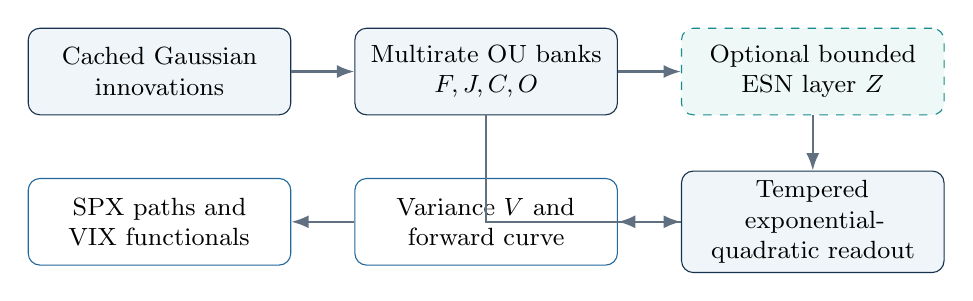
\begin{tikzpicture}[
  node distance=7mm and 8mm,
  box/.style={draw=navy,rounded corners=1.5mm,fill=pale,align=center,
              minimum height=11mm,text width=31mm,font=\small},
  opt/.style={draw=teal,dashed,rounded corners=1.5mm,fill=paleteal,align=center,
              minimum height=11mm,text width=31mm,font=\small},
  outputbox/.style={draw=blue,rounded corners=1.5mm,fill=white,align=center,
              minimum height=11mm,text width=31mm,font=\small},
  arr/.style={-{Latex[length=2.2mm]},thick,color=muted}
]
\node[box] (shocks) {Cached Gaussian\\innovations};
\node[box,right=of shocks] (ou) {Multirate OU banks\\\(F,J,C,O\)};
\node[opt,right=of ou] (esn) {Optional bounded\\ESN layer \(Z\)};
\node[box,below=of esn] (readout) {Tempered exponential-\\quadratic readout};
\node[outputbox,left=of readout] (variance) {Variance \(V\) and\\forward curve};
\node[outputbox,left=of variance] (claims) {SPX paths and\\VIX functionals};
\draw[arr] (shocks)--(ou);
\draw[arr] (ou)--(esn);
\draw[arr] (ou)|-(readout);
\draw[arr] (esn)--(readout);
\draw[arr] (readout)--(variance);
\draw[arr] (variance)--(claims);
\end{tikzpicture}
\end{center}

\section{Parameter hierarchy and path reuse}

\subsection{Hyperparameters, structural parameters and daily inputs}

\begin{longtable}{@{}L{32mm}L{52mm}L{58mm}@{}}
\toprule
\textbf{Class} & \textbf{Examples} & \textbf{Treatment} \\
\midrule
\endfirsthead
\toprule
\textbf{Class} & \textbf{Examples} & \textbf{Treatment} \\
\midrule
\endhead
Architectural hyperparameters
& Bank dimensions; OU rate grids; reservoir matrices \(A_Z,B_Z\); leak \(\alpha\);
feature map \(\psi\); cap family
& Selected in an outer validation loop and changed infrequently. Changing OU rates or fixed
reservoir weights requires rebuilding state features. \\
\addlinespace
Shared structural parameters
& \(a,f,c_C,q_Z,\beta,q_J,q_O,\delta,\rho_F,\rho_J\)
& Estimated from a panel of physical and option data with regularisation. Readout changes do
not change cached states; correlation changes require rebuilding correlated states from the
same primitive innovations. \\
\addlinespace
Measure-dependent parameters
& \(\theta\) and unspanned components of \(\gamma\)
& Thin deterministic parameterisation. They shift conditional means but do not change OU
covariances. \\
\addlinespace
Daily inputs and states
& \(\xi_0(\cdot)\), rates, dividends, spot, filtered \(X_t,Z_t\)
& Updated daily. They are inputs or filtered states, not structural calibration parameters. \\
\bottomrule
\end{longtable}

\subsection{What path reuse does and does not mean}

For fixed hyperparameters and correlations, simulate or reconstruct once:

\begin{equation}
\left\{\Delta W^S,\Delta B^F,\Delta B^J,\Delta B^C,\Delta B^O;\ X;\ Z\right\}.
\end{equation}

When \(q_Z,\beta,q_J,q_O,c_C,\delta\) or the deterministic risk premia change, no new random
numbers are required. The readout, variance, stock integral and payoffs must nevertheless be
recomputed. It is impossible for the final \(S\) or \(\VIX\) paths to remain unchanged when
the volatility readout changes.

\begin{center}
\begin{tabularx}{\textwidth}{@{}Y C{28mm} Y@{}}
\toprule
\textbf{Change} & \textbf{New random draw?} & \textbf{Required recomputation} \\
\midrule
Readout coefficient & No & \(\eta,V,S\), VIX map and payoffs \\
Deterministic risk premium & No & Deterministic OU mean shift; possibly \(Z\); then pricing quantities \\
Forward-variance curve & No & Variance level, \(S\), VIX and payoffs \\
Correlation & No, if primitive shocks are cached & Correlated drivers and affected OU states \\
OU rate grid or reservoir matrix & No new seed is necessary, but the state changes & Full feature-engine reconstruction \\
\bottomrule
\end{tabularx}
\end{center}

This is the same computational principle exploited by precomputed signature and quantisation
approaches: expensive stochastic input is generated offline, while parameter-dependent maps
are evaluated during optimisation \cite{cuchiero2024,abijaber2024}.

\section{Physical-measure stylised facts}

The selected targets are standard empirical regularities of equity markets, with roughness and
time-reversal asymmetry adding more discriminating requirements to the classical inventory
\cite{cont2001,gatheral2018,zumbach2009}.

\subsection{Negligible linear autocorrelation of returns}

For non-overlapping increments over a short interval \(\Delta\), the martingale part of
\cref{eq:stock-P} has conditional mean zero and variance of order \(\Delta\). The predictable
return component is of order \(\Delta\), so its contribution to return covariance is of order
\(\Delta^2\). Consequently, linear return autocorrelation is small at intraday and daily
frequencies unless the risk-premium term is made too large or too state dependent.

Under \(\Qq\), discounted simple gains are martingale increments and therefore orthogonal
across non-overlapping intervals. Log returns need not be exactly uncorrelated because their
drift contains \(-V_t/2\).

\textbf{Status: P/O.} Near-zero autocorrelation is structurally natural, not an identity under
\(\Pp\). It must remain an explicit diagnostic, especially after estimating \(\theta\).

\subsection{Volatility clustering}

The recommended architecture obtains clustering from the exogenous slow bank rather than the
endogenous activity filter. If \(C_t=c_C^\top X_t^C\) and the coordinates are independent
stationary OU processes, then

\begin{equation}
\Cov(C_t,C_{t+\tau})
=\sum_{j=1}^{N_C}c_{C,j}^2e^{-\lambda_j^C\tau}.
\label{eq:cluster-cov}
\end{equation}

A geometrically spaced rate grid approximates slowly decaying covariance over a prescribed
finite interval. The monotone exponential link transfers persistence from \(\eta\) to \(V\);
quadratic channels add modes with decay rates such as \(2\lambda_j\) and
\(\lambda_i+\lambda_j\).

This choice preserves strong frozen-state reuse. An endogenous activity bank

\begin{equation}
\dd\Sigma_{k,t}=\alpha_k(V_t-\Sigma_{k,t})\dd t
\end{equation}

remains an optional challenger if the exogenous bank cannot fit the empirical volatility ACF.
It needs no new random numbers, but it must be recomputed whenever the readout changes.

\textbf{Status: C/P/O.} Persistence is built into the rate mixture; matching its empirical
magnitude and shape is a calibration question.

\subsection{Finite-scale roughness}

Rough volatility is usually expressed through the small-lag scaling

\begin{equation}
\E\!\left[\bigl(\log V_{t+\tau}-\log V_t\bigr)^2\right]
\asymp C\tau^{2H},\qquad H<\frac12,
\label{eq:rough-scaling}
\end{equation}

with empirical estimates often near \(H=0.1\) \cite{gatheral2018}. A fractional kernel can be
approximated on a chosen range by a positive exponential sum,

\begin{equation}
K_H(t)\approx\sum_{j=1}^{N_F}a_je^{-\lambda_j^F t},
\label{eq:kernel-lift}
\end{equation}

which is precisely a Markovian OU lift \cite{abijaber2019}. The feedback projection
\(Y=a^\top X^F\) therefore reproduces \cref{eq:rough-scaling} over the frequencies covered by
the rate grid.

If \(g\) is the smooth map from the state to log variance, then

\begin{equation}
g(Y_{t+\tau})-g(Y_t)
=g'(Y_t)(Y_{t+\tau}-Y_t)+o_{\Pp}(\tau^H).
\end{equation}

Thus the exponent is locally preserved whenever \(g'(Y_t)\neq0\). The derivative can vanish
at the parabola vertex and becomes small near cap saturation, so roughness should be estimated
on the bulk of the volatility distribution.

\begin{warningbox}[Finite lift, finite claim]
Every finite OU system is a semimartingale and has Brownian \(H=1/2\) behaviour at sufficiently
small asymptotic lags. The defensible claim is rough behaviour on the intraday-to-daily scale
range selected by \([\lambda_{\min}^F,\lambda_{\max}^F]\), not genuine fractional asymptotics
at arbitrarily small times.
\end{warningbox}

\textbf{Status: P/O.} The lift supports the target scaling over a finite band; the realised
band and estimated \(H\) must be verified with a noise-robust realised-volatility estimator.

\subsection{Leverage effect}

For a lag \(\tau>0\), define the leverage statistic

\begin{equation}
L(\tau)=\Corr_{\Pp}\!\left(r_t,V_{t+\tau}\right),
\qquad L(\tau)<0\ \text{empirically}.
\end{equation}

The feedback contribution is \(q_Z(Y-\beta)^2\), with derivative

\begin{equation}
\frac{\partial\eta}{\partial Y}=2q_Z(Y-\beta).
\end{equation}

Near the stationary centre \(Y\approx0\), its sign is \(-\operatorname{sign}(q_Z\beta)\). Since
the outer link is increasing away from cap saturation, the instantaneous return--log-variance
covariation has leading sign

\begin{equation}
\operatorname{sign}\!\left(\dd\langle \log S,\log V\rangle_t\right)
\approx -\operatorname{sign}(q_Z\beta\rho_F).
\label{eq:leverage-sign}
\end{equation}

Under the present convention, \(q_Z>0\), \(\beta>0\), \(\rho_F>0\) therefore produce negative
leverage. This apparently unusual positive correlation is a consequence of the shifted
parabola convention; reversing both \(\beta\) and \(\rho_F\) leaves the local sign unchanged.

The shift is essential. With \(\beta=0\), the quadratic channel is locally even around the
stationary centre and does not generate a stable directional leverage effect. The fast bank
should not dominate total variance, because a large orthogonal or symmetric component dilutes
correlation-based leverage statistics.

\textbf{Status: P/N/O.} The sign mechanism is explicit and has been observed in the programme's
simulations. Its empirical magnitude remains a calibration constraint.

\subsection{Strong Zumbach effect}

The Zumbach effect is a causal time-reversal asymmetry between past returns and future
volatility. A representative statistic at horizon \(\tau\) is

\begin{equation}
Z(\tau)
=\Corr\!\left(R_{t-\tau,t}^2,\operatorname{RV}_{t,t+\tau}\right)
-\Corr\!\left(\operatorname{RV}_{t-\tau,t},R_{t,t+\tau}^2\right).
\label{eq:zumbach}
\end{equation}

A reversible exogenous volatility process independent of returns has \(Z(\tau)=0\) in the
ideal stationary limit. The current model breaks reversibility without making the OU driver
amplitude depend on \(V\):

\begin{enumerate}
  \item the feedback state is a causal filter of a shock correlated with the return innovation;
  \item the future variance depends quadratically on that state;
  \item past return shocks therefore affect future variance through \(Y^2\), while the
  time-reversed pairing does not have the same causal construction.
\end{enumerate}

The programme's controlled Gate C experiment provides mechanism evidence:

\begin{center}
\begin{tabularx}{0.90\textwidth}{@{}Y C{38mm}@{}}
\toprule
\textbf{Configuration} & \textbf{Pearson asymmetry} \\
\midrule
GARCH positive control & \(0.118\pm0.009\) \\
Standardised correlated driver, quadratic readout & \(0.297\pm0.011\) \\
Quadratic-ablation reference run & \(0.215\pm0.018\) \\
Same ablation run with \(q_Z=0\) & \(0.000\pm0.002\) \\
\bottomrule
\end{tabularx}
\end{center}

These are replicated mechanism checks, not market calibration results. They show that the
quadratic readout is load-bearing and that variance-dependent raw-return driving is not
required. The standardised-driver sweep and the quadratic ablation used different reference
runs, so their absolute levels should not be compared as if they were one nested sample. This
differs from endogenous price-feedback models such as quadratic rough Heston, but it targets
the same time-reversal asymmetry \cite{zumbach2009,gatheral2020}.

\begin{warningbox}[Measurement requirement]
In the programme's validation, replacing realised variance by daily squared returns removed
almost all power of the Zumbach statistic, even on a GARCH positive control. The empirical
target should therefore use intraday realised variance, and every result should be accompanied
by a reversible null, a positive control and replication uncertainty.
\end{warningbox}

\textbf{Status: N/O.} The mechanism is strongly supported by ablation. Its market magnitude
cannot be claimed before a correctly measured intraday-data study.

\subsection{Heavy-tailed returns at relevant frequencies}

Conditional on the variance path, short-horizon returns are approximately Gaussian; their
unconditional distribution is a variance mixture. The exponential-quadratic channel produces
large finite-frequency dispersion. In the scalar untempered illustration

\begin{equation}
\sigma=e^{qY^2},\qquad Y\sim\mathcal N(0,1),\qquad q>0,
\end{equation}

one has, up to a slowly varying logarithmic factor,

\begin{equation}
\Pp(\sigma>x)
=\Pp\!\left(Y^2>\frac{\log x}{q}\right)
\asymp x^{-1/(2q)}(\log x)^{-1/2}.
\label{eq:scalar-tail}
\end{equation}

This explains why an exponential quadratic can generate much heavier observable tails than a
direct quadratic variance map. It does not, by itself, establish the tail index of a
continuous-time return when the volatility state and return share Brownian increments.

For \(X\sim\mathcal N(m,\Sigma)\) and a quadratic matrix \(Q\), the untempered first variance
moment requires

\begin{equation}
I-4\Sigma^{1/2}Q\Sigma^{1/2}\succ0.
\label{eq:moment-domain}
\end{equation}

Higher variance moments impose progressively stronger spectral conditions. The tempered link
removes asymptotic moment explosion and replaces true power tails by a broad but ultimately
truncated mixture. This is consistent with the stated objective: realistic heavy-tail
behaviour over observable intraday and daily quantiles is more important than an exact
asymptotic law.

The optional orthogonal block can increase log-volatility dispersion without changing the
largest quadratic eigenvalue when its loading is spread over many independent directions and
each new eigenvalue remains below the existing maximum. It should be activated only if the
correlated feedback and fast banks cannot match return kurtosis and volatility quantiles
without damaging leverage or Zumbach.

\textbf{Status: P/N/O.} Heavy finite-frequency tails are a strong capability of the readout.
Their quantitative fit and stability across aggregation horizons remain empirical tests.

\subsection{Taylor effect}

The Taylor effect requires

\begin{equation}
\Corr(|r_t|,|r_{t+k}|)
>\Corr(r_t^2,r_{t+k}^2)
\label{eq:taylor-def}
\end{equation}

over a relevant set of lags. It is not implied by leverage, roughness or clustering alone.
For the benchmark representation \(r_t=e^{X_t}\varepsilon_t\), where \(X\) is stationary
Gaussian with variance \(s^2\), lag correlation \(\rho_k\), and
\(\varepsilon_t\stackrel{\mathrm{iid}}{\sim}\mathcal N(0,1)\), direct calculation gives

\begin{align}
\rho_{|r|}(k)
&=\frac{(2/\pi)\left(e^{s^2\rho_k}-1\right)}
        {e^{s^2}-2/\pi}, \\
\rho_{r^2}(k)
&=\frac{e^{4s^2\rho_k}-1}{3e^{4s^2}-1}.
\label{eq:taylor-formula}
\end{align}

At small \(s^2\), the first correlation grows more slowly, so the Taylor inequality fails.
At \(\rho_k=0.9\), the crossover in this benchmark is approximately
\(s^2=0.081\), or \(\operatorname{sd}(\log\sigma)\approx0.285\). The threshold changes with
persistence and with departures from the Gaussian log-volatility benchmark.

The exponential-quadratic and optional multi-directional blocks provide the required
dispersion more naturally than a direct quadratic variance readout. Nevertheless, Taylor must
remain a diagnostic or low-weight target rather than a theorem of the architecture.

\textbf{Status: P/N/O.} The model can cross the analytically identified dispersion threshold;
the sign and lag range must be checked after every joint calibration.

\subsection{Fast volatility, downside asymmetry and VIX spike relaxation}

Suppose a fast OU projection is shocked to \(F_t=f_0\). Ignoring subsequent noise,

\begin{equation}
F_{t+s}\approx f_0e^{-\lambda_Js}.
\end{equation}

Its untempered contribution to relative variance is

\begin{equation}
\frac{V_{t+s}}{\bar V_{t+s}}
\approx\exp\!\left(
2q_J\left[f_0^2e^{-2\lambda_Js}-2\beta_Jf_0e^{-\lambda_Js}\right]
\right),
\label{eq:spike-path}
\end{equation}

where \(\bar V\) uses the resting fast state \(F=0\). For equal-magnitude shocks \(f>0\),

\begin{equation}
\log\!\frac{V(F=-f)}{V(F=+f)}=8q_J\beta_Jf.
\label{eq:spike-asymmetry}
\end{equation}

Thus \(q_J>0\), \(\beta_J>0\), and positive fast-bank/equity correlation make a negative
equity shock produce a larger contemporaneous volatility response than an equal positive
shock. The result is exact below the tempering region; the smooth cap can attenuate it in the
far tail. The zero-shift restriction is the symmetric nested control.

The corresponding time derivative is

\begin{equation}
\frac{\dd}{\dd s}\log\!\left(\frac{V_{t+s}}{\bar V_{t+s}}\right)
=-4\lambda_Jq_J\left[
f_0^2e^{-2\lambda_Js}-\beta_Jf_0e^{-\lambda_Js}
\right].
\label{eq:spike-decay}
\end{equation}

For the downside shocks of interest (\(f_0<0\)), this derivative is negative and its magnitude
is largest near the event before slowing progressively. Several fast and medium OU rates create
a sharp front followed by a persistent shoulder. This temporal shape comes from the interaction
of mean reversion with the exponential level map, not from a jump in the state process.

\begin{resultbox}[Fresh-seed mechanism screen]
A paired screen of 16 previously selected configuration--scenario pairs, five fresh seeds and
six values \(\beta_J\in\{0,0.1,\ldots,0.5\}\) produced 480 evaluations. At \(\beta_J=0.1\),
the downside-minus-upside median day-zero volatility-response gap increased from 35.0\% to
38.7\%, and the corresponding days 1--5 gap increased from 29.4\% to 37.3\%. All seven
pre-existing stylised-fact proxy gates passed in 67 of 80 evaluations; six of 16 configurations
passed on every fresh seed. All failures at this shift came from the positive-Zumbach lower
bound. This is controlled synthetic mechanism evidence, not an empirical SPX calibration.
\end{resultbox}

The cap may flatten the very top of an extreme spike. Its level should be selected so that it
almost never binds in the calibration region while still controlling martingality outside it.

\textbf{Status: P/N/O.} The relaxation shape follows from the model and the downside orientation
has controlled numerical support. Matching the distribution,
amplitude and equity co-movement of observed VIX spikes is an empirical requirement.

\subsection{Summary of physical-measure support}

\begin{longtable}{@{}L{34mm}C{20mm}L{88mm}@{}}
\toprule
\textbf{Target} & \textbf{Status} & \textbf{Load-bearing component} \\
\midrule
\endfirsthead
\toprule
\textbf{Target} & \textbf{Status} & \textbf{Load-bearing component} \\
\midrule
\endhead
Near-zero return ACF & P/O & Diffusive return innovation and parsimonious deterministic Sharpe ratio \\
Volatility clustering & C/P/O & Slow exogenous OU mixture \\
Finite-scale roughness & P/O & Shared-driver rough OU lift and appropriate rate grid \\
Leverage & P/N/O & Shift \(\beta\), curvature \(q_Z\), and return correlation \(\rho_F\) \\
Strong Zumbach & N/O & Causal correlated OU filter plus quadratic readout \\
Heavy finite-frequency tails & P/N/O & Exponential quadratic; optional orthogonal dispersion block \\
Taylor effect & P/N/O & Sufficient log-volatility dispersion and persistence \\
Fast asymmetric VIX-like spikes & P/N/O & Shifted fast, partly correlated OU projection in the exponential quadratic \\
\bottomrule
\end{longtable}

\section{Risk-neutral pricing and joint SPX--VIX calibration}

\subsection{Forward variance, VIX and VIX futures}

By \cref{eq:variance}, the input curve satisfies

\begin{equation}
\E_0^{\Qq}[V_t]=\xi_0(t).
\end{equation}

For a VIX window \(\Delta=30/365\), ignoring the conventional discrete-sampling and corridor
adjustments,

\begin{equation}
\VIX_T^2
=\frac{100^2}{\Delta}\int_T^{T+\Delta}
\E_T^{\Qq}[V_u]\dd u.
\label{eq:vix}
\end{equation}

Matching \(\xi_0\) does not automatically match VIX futures, because

\begin{equation}
F_0^{\VIX}(T)=\E_0^{\Qq}[\VIX_T]
\leq\sqrt{\E_0^{\Qq}[\VIX_T^2]}.
\end{equation}

The difference is the VIX convexity adjustment and must be calibrated or reported, not hidden
inside the forward-variance normalisation.

\subsection{Analytic Gaussian-core moments}

If \(\delta=0\) and \(h(x)=x\), the OU state is conditionally Gaussian and the score is
quadratic. If

\begin{equation}
X_u\mid\F_T\sim\mathcal N(m_{T,u},\Sigma_{T,u})
\end{equation}

and the exponent is \(X^\top AX+b^\top X+c\), then

\begin{align}
&\E_T\!\left[e^{X^\top AX+b^\top X+c}\right] \\
&\quad=
\frac{\exp\!\left(
c+m^\top Am+b^\top m
+\tfrac12(2Am+b)^\top(I-2\Sigma A)^{-1}\Sigma(2Am+b)
\right)}
{\sqrt{\det(I-2\Sigma A)}},
\label{eq:gaussian-quadratic}
\end{align}

provided

\begin{equation}
I-2\Sigma^{1/2}A\Sigma^{1/2}\succ0.
\end{equation}

This turns \cref{eq:vix} into a one-dimensional deterministic maturity quadrature evaluated
at the cached state \(X_T\). No nested Monte Carlo is needed in the Gaussian shadow model.

\subsection{Tempering and the nonlinear ESN layer}

The recommended tempered model does not retain the closed form
\cref{eq:gaussian-quadratic}. Neither does the full model with \(\delta\neq0\). It remains
computationally tractable through one of the following offline--online decompositions:

\begin{enumerate}
  \item low-dimensional Gauss--Hermite or sparse-grid quadrature when the active quadratic
  directions are few;
  \item functional quantisation of the Gaussian state;
  \item least-squares conditional expectation on cached states;
  \item a neural surrogate trained on the state and parameter domain, with the Gaussian core
  used as a control variate.
\end{enumerate}

Quantisation and neural pricing have already been demonstrated for Gaussian polynomial
SPX--VIX models \cite{abijaber2024}; precomputed signature samples provide another successful
offline calibration paradigm \cite{cuchiero2024}. These are useful numerical templates, not
proofs that the present model will calibrate.

\subsection{SPX pricing and martingality}

For fixed cached innovations and a candidate parameter vector, compute

\begin{equation}
\log\frac{S_T}{S_0}
=\int_0^T\left(r_t-d_t-\frac12V_t\right)\dd t
+\int_0^T\sqrt{V_t}\dd W_t^{S,\Qq}.
\end{equation}

The discounted stock is always a nonnegative local martingale. It is a true martingale if the
stochastic exponential has expectation one. In the tempered model, \(V\) is bounded on every
finite horizon when \(\xi_0\) and the deterministic risk premia are bounded and the positive
normaliser \(M_{\Qq}\) is bounded away from zero. Novikov's condition then gives

\begin{equation}
\E^{\Qq}\!\left[
\exp\!\left(\frac12\int_0^T V_t\dd t\right)
\right]<\infty,
\end{equation}

so the discounted stock is a true martingale. In the untempered, return-correlated
exponential-quadratic model, finite marginal moments do not by themselves establish true
martingality; the admissible domain must be analysed separately.

\begin{resultbox}[Production choice]
The smooth upper tempering is part of the recommended model, not merely a numerical emergency
stop. It provides a clean finite-horizon martingale argument while preserving the untempered
map over the empirically relevant state region.
\end{resultbox}

\subsection{Why a quintic polynomial is not structurally required}

The fifth-degree polynomial used by Abi Jaber, Illand and Li is effective in their
one-factor Gaussian polynomial family and helps generate upward VIX smiles
\cite{abijaber2024}. It is not a necessity theorem. Two complementary results make this clear:

\begin{itemize}
  \item quadratic rough Heston combines a quadratic variance map with rough feedback and
  provides a continuous-path solution to the joint SPX--VIX smile problem
  \cite{gatheral2020};
  \item signature models obtain strong joint calibrations using several low-order path
  features rather than a scalar quintic readout \cite{cuchiero2024}.
\end{itemize}

The present architecture substitutes feature diversity, rate diversity and exponential
convexity for scalar polynomial degree. Its fast and slow quadratic directions have distinct
economic roles, which should improve identifiability relative to an unrestricted high-degree
polynomial.

\section{Joint calibration programme}

\subsection{Recommended nested sequence}

\begin{center}
\begin{tabularx}{\textwidth}{@{}C{13mm}L{40mm}Y@{}}
\toprule
\textbf{Model} & \textbf{Readout} & \textbf{Purpose} \\
\midrule
M0 & Positive direct quadratic variance & Minimal baseline; tests whether exponential
convexity is genuinely needed. \\
M1 & Untempered Gaussian exponential quadratic, \(\delta=0\) & Analytic shadow model;
moment-domain and VIX-control-variate benchmark. \\
M2 & Tempered Gaussian exponential quadratic, \(\delta=0\) & Recommended production core. \\
M3 & M2 plus \(\delta^\top Z\) & Activate only if the nonlinear ESN layer materially improves
out-of-sample physical facts or option errors. \\
M4 & M3 plus orthogonal block \(q_O>0\) & Optional finite-frequency dispersion and tail tuning;
activate only after diagnosing a residual deficiency. \\
\bottomrule
\end{tabularx}
\end{center}

If M2 cannot reproduce synthetic surfaces generated by a quintic OU benchmark, add a second
identified quadratic direction before increasing polynomial degree. This directly tests the
hypothesis that factor diversity can replace degree.

\subsection{Relation of M2 to ESN--A2}
\label{sec:m2-versus-a2}

M2 is a structured descendant of ESN--A2, but it is neither a renaming nor a nested
restriction of A2. The common core is a fixed multirate Gaussian reservoir whose state can be
reused while the volatility readout changes. The redesign concerns the organisation of that
state, the readout parameterisation, and the separation between physical and pricing inputs.
The comparison below refers to the supplied reconstructed A2 engine; its implementation file
records that it was reconstructed after an environment reset and validated against the reported
roughness targets. Consequently, code-specific A2 conclusions carry that provenance.

\newpage
\begin{samepage}
On a grid of width \(\Delta\), the A2 rough bank and nonlinear layer can be written schematically
as

\begin{align}
r_{n+1}
  &=D_{\lambda}r_n+c_{\lambda}\varepsilon_{n+1},
  &D_{\lambda,jj}&=e^{-\lambda_j\Delta},
  &c_{\lambda,j}&=\sqrt{1-e^{-2\lambda_j\Delta}}, \\
z_{n+1}
  &=\Phi_{\mathrm{A2}}(r_{n+1},z_n),
\end{align}
\end{samepage}

where the same scalar innovation \(\varepsilon_{n+1}\) drives every coordinate of \(r\) and the
equity return in the supplied simulator. The map \(\Phi_{\mathrm{A2}}\) is the leaky, bounded
second layer built from quadratic and linear features, a hyperbolic tangent, local recurrence,
and the state-dependent norm gate. Its volatility score and variance map are

\begin{align}
\eta_n^{\mathrm{A2}}
  &=b_0+\kappa q^\top r_n+w_z^\top z_n
    +\frac{m_1}{N_r}\lVert r_n\rVert^2
    +\frac{m_2}{N_r}(q^\top r_n)^2,
\label{eq:a2-readout}\\
V_n^{\mathrm{A2}}
  &=\sigma_{\min}^2+\operatorname{softplus}
    \!\left(\eta_n^{\mathrm{A2}}\right)^2.
\label{eq:a2-variance}
\end{align}

At the A2 resting bias, softplus is already close to its exponential branch. Thus A2 already
contains the central idea ``Gaussian reservoir plus approximately exponential-quadratic
readout.'' In contrast, M2 sets \(\delta=q_O=0\) in \cref{eq:eta} and uses

\begin{align}
\eta_t^{\mathrm{M2}}
  &=c_C^\top X_t^C+q_Z(Y_t-\beta)^2+q_J(F_t-\beta_J)^2,
\label{eq:m2-readout-comparison}\\
V_t^{\mathrm{M2}}
  &=\underline v+\bigl(\xi_0(t)-\underline v\bigr)
    \frac{G_{L,\kappa}(\eta_t^{\mathrm{M2}})}{M_{\Qq}(t)}.
\label{eq:m2-variance-comparison}
\end{align}

The models therefore share a mathematical backbone, but they are not the same parameterised
family:

\small
\begin{longtable}{@{}L{25mm}L{56mm}L{56mm}@{}}
\toprule
\textbf{Component} & \textbf{ESN--A2} & \textbf{M2} \\
\midrule
\endfirsthead
\toprule
\textbf{Component} & \textbf{ESN--A2} & \textbf{M2} \\
\midrule
\endhead
State drivers
& One multirate rough bank driven by the equity innovation; the coupling is effectively
perfect in the supplied engine.
& Separate feedback, fast-spike, and clustering banks. Feedback and spike shocks may be only
partially correlated with the equity shock; clustering shocks are independent. \\
\addlinespace
Nonlinear layer
& The bounded recurrent \(z\)-layer contributes directly through \(w_z^\top z\).
& Inactive: \(\delta=0\). M3, not M2, restores an optional fixed contractive echo layer. \\
\addlinespace
Leverage and Zumbach
& The linear rough projection, aligned quadratic projection, and nonlinear layer have
overlapping effects, so attribution is parameter-regime dependent.
& Concentrated in the shifted correlated channel \(q_Z(Y-\beta)^2\), whose slope controls the
leverage sign and whose state dependence generates time-reversal asymmetry. \\
\addlinespace
Clustering
& Encoded jointly by the multirate bank, especially its isotropic reservoir-energy term, and
persistence transmitted through the nonlinear layer.
& A dedicated slow linear bank \(c_C^\top X^C\), separated from the leverage--Zumbach channel. \\
\addlinespace
Fast VIX-like spikes
& No separately identified fast-spike bank.
& A dedicated convex direction \(q_J(F-\beta_J)^2\), with its own fast rate grid and return
correlation; \(\beta_J>0\) orients equal-magnitude responses toward downside shocks. \\
\addlinespace
Variance map and tails
& Squared softplus with an unbounded exponential branch; the quadratic eigenvalues govern its
asymptotic moment domain.
& A direct exponential-quadratic shadow map, smoothly tempered in production and close to the
shadow map below the cap. The target is finite-frequency fat tails, not an asymptotic power law. \\
\addlinespace
Measure change
& The supplied engine is a physical-measure simulator and does not give a complete, separately
normalised \(\Pp/\Qq\) specification.
& Explicit \(\Pp\) and \(\Qq\) stock equations, deterministic Girsanov kernel, unspanned risk
premia, and a market forward-variance normalisation. \\
\addlinespace
Path reuse
& Available while parameters that determine \(r\) and \(z\) are fixed; changing reservoir or
second-layer parameters rebuilds the state.
& Primitive shocks and exogenous states are cached. Readout, forward-curve, and deterministic
risk-premium changes require deterministic state adjustments and revaluation, but no new
random draw. \\
\addlinespace
Calibration roles
& The audited parameter split allowed quantities intended for daily recalibration to move most
of the physical statistics.
& Architecture, shared structural parameters, measure-dependent premia, and daily inputs are
separated explicitly; shared readout coefficients cannot be overwritten by a daily \(\Qq\) fit. \\
\bottomrule
\end{longtable}
\normalsize

The shifted M2 channel makes the relationship particularly transparent:

\begin{equation}
q_Z(Y-\beta)^2=q_ZY^2-2q_Z\beta Y+q_Z\beta^2.
\label{eq:m2-shift-expansion}
\end{equation}

It combines A2's aligned linear and quadratic rough-factor channels, but imposes the identified
coefficient relation \(\kappa_Y=-2q_Z\beta\) after normalisation. Conversely, baseline M2 drops
A2's isotropic energy and nonlinear readouts, replaces their clustering role by \(X^C\), and
adds the fast direction \(F\). M4 can restore an independent quadratic dispersion channel, but
that channel lives in an orthogonal bank and is therefore not equivalent to A2's
\(\lVert r\rVert^2\). M3 restores nonlinear memory, but its controlled echo layer does not make
the resulting model identical to A2 either.

\begin{resultbox}[Nesting statement]
A2 is not a parameter point of M2, and M2 is not a parameter point of A2. M2 is best viewed as
a lower-nonlinearity but more economically structured redesign of A2. It retains the exogenous
Gaussian and exponential-quadratic mechanisms, while changing the driver topology, assigning
separate channels to clustering and spikes, enforcing path-reuse discipline, and adding the
objects required for joint SPX--VIX pricing.
\end{resultbox}

The transfer of stylised-fact evidence is therefore conditional. A2 experiments motivate the
rough-reservoir and convex-readout mechanisms, but they do not prove that M2 preserves their
empirical magnitudes. M2 must be evaluated on its own with matched estimators, multiple seeds,
and the ablations prescribed below. Likewise, M2 has better specified joint-pricing capacity,
not a demonstrated SPX--VIX fit in the absence of option data.

\subsection{Calibration hierarchy}

Let \(\Theta_H\), \(\Theta_S\), \(\Theta_M\) and \(D_t\) denote architectural
hyperparameters, shared structural parameters, measure-dependent parameters and daily inputs.
A practical hierarchy is:

\begin{enumerate}
  \item \textbf{Architecture selection.} Choose dimensions and rate grids using rolling
  physical-measure validation and synthetic option-capacity tests. This is the expensive outer
  loop.
  \item \textbf{Shared structural estimation.} Estimate \(\Theta_S\) from historical windows
  and a panel of option surfaces, with stability penalties across dates.
  \item \textbf{Measure change.} Estimate the thin deterministic unspanned risk premia in
  \(\Theta_M\), with \(\theta\) pinned by the physical drift convention.
  \item \textbf{Daily calibration.} Strip \(\xi_0\), filter the current state and calibrate only
  the permitted daily pricing quantities.
\end{enumerate}

Because shared readout parameters affect both \(\Pp\) and \(\Qq\), a purely sequential
"fit \(\Pp\), then overwrite under \(\Qq\)" procedure is not valid. Use either a joint loss
or alternating minimisation with a physical-measure retention penalty:

\begin{equation}
\mathcal L(\Theta)
=w_P\mathcal L_P
+w_S\mathcal L_{\mathrm{SPX}}
+w_V\mathcal L_{\mathrm{VIX}}
+w_F\mathcal L_{\mathrm{VIX\ futures}}
+\mathcal R(\Theta).
\label{eq:joint-loss}
\end{equation}

Option residuals should be expressed in bid--ask-normalised prices, for example

\begin{equation}
\varepsilon_i
=\frac{C_i^{\mathrm{model}}-C_i^{\mathrm{mid}}}
{\max\{\tfrac12(C_i^{\mathrm{ask}}-C_i^{\mathrm{bid}}),\epsilon_i^{\mathrm{floor}}\}},
\end{equation}

rather than unweighted implied-volatility errors. VIX futures must be included separately from
the forward-variance curve.

\subsection{Validation and falsification tests}

\begin{longtable}{@{}L{38mm}L{52mm}L{52mm}@{}}
\toprule
\textbf{Question} & \textbf{Required test} & \textbf{Failure implication} \\
\midrule
\endfirsthead
\toprule
\textbf{Question} & \textbf{Required test} & \textbf{Failure implication} \\
\midrule
\endhead
Roughness & Structure functions on noise-robust intraday realised volatility across the
designed lag band & Retune rate grid; do not add readout degree. \\
Leverage & Lagged return--realised-volatility correlation with confidence bands & Adjust
\(\beta,\rho_F\), or add a separate linear leverage bank. \\
Zumbach & Realised-variance statistic, reversible null, positive control, multiple seeds or
blocks & Reassess the correlated quadratic mechanism or measurement protocol. \\
Heavy tails & QQ/body fit, kurtosis, threshold-stability plots and aggregation horizons & Add
orthogonal dispersion only after excluding measurement and cap effects. \\
Taylor & Both correlation curves and the log-volatility dispersion threshold & Treat as
secondary unless failure contaminates more important targets. \\
VIX spikes & Peak amplitude, rise/decay asymmetry and SPX co-movement & Retune fast rates and
\(\rho_J\); avoid a dominant independent spike factor. \\
Martingale & Analytic boundedness proof plus Monte Carlo defect within sampling error & Reject
parameter point or lower the cap. \\
Joint surface capacity & Bid--ask-normalised SPX/VIX errors and VIX-futures errors over dates &
Add a second quadratic direction before quintic degree. \\
Path reuse & Bitwise equality of cached \(X,Z\) under readout perturbations & Implementation
violates the architectural constraint. \\
\bottomrule
\end{longtable}

\section{Open issues and limitations}

\begin{unresolvedbox}[What is not yet established]
\begin{enumerate}
  \item No SPX/VIX option data have yet been used, so joint calibration capacity is untested.
  \item Identifiability of curvature, shift, correlations, fast rates and deterministic risk
  premia must be studied through Jacobian singular values, profile likelihoods and rolling
  stability.
  \item The optimal cap level must balance negligible in-sample binding against robust moment
  and martingale control.
  \item A finite OU lift produces only finite-scale roughness.
  \item The exact market magnitude of the Zumbach effect requires intraday realised variance;
  daily squared returns are an inadequate proxy for the current statistic.
  \item The nonlinear second layer is not currently justified by the Gate C Zumbach ablation.
  It must earn its parameters through out-of-sample improvement.
\end{enumerate}
\end{unresolvedbox}

Three interactions deserve particular monitoring:

\begin{itemize}
  \item Increasing an independent dispersion block can improve tails and Taylor while diluting
  leverage and Zumbach correlations.
  \item Increasing the correlated quadratic curvature strengthens Zumbach and tails but pushes
  the untempered model toward moment and martingale boundaries.
  \item A low cap improves safety but can flatten extreme VIX spikes, distort roughness
  estimates in the upper tail and limit the VIX smile.
\end{itemize}

These are not arguments against the model. They are the principal trade-offs that the joint
objective must expose rather than hide.

\section{Conclusion}

The current candidate is a two-layer exogenous reservoir architecture with a recommended
Gaussian first calibration and an optional nonlinear ESN extension. Its defining choices are:

\begin{itemize}
  \item multirate OU banks with variance-independent drivers;
  \item a return-correlated rough feedback projection;
  \item a shifted quadratic feedback term for leverage and Zumbach;
  \item slow exogenous modes for clustering and path reuse;
  \item a shifted fast, partly return-correlated direction for downside-oriented VIX spike
  relaxation, nested at \(\beta_J=0\);
  \item a normalised, smoothly tempered exponential-quadratic variance map;
  \item a deterministic market price of risk preserving the Gaussian OU class under \(\Qq\);
  \item an optional independent dispersion block and optional nonlinear ESN layer, both subject
  to ablation.
\end{itemize}

This construction retains the mechanisms needed for the targeted physical-measure facts and
offers a viable offline--online route to SPX/VIX calibration without a quintic polynomial.
Roughness and path reuse are architectural; leverage has an explicit sign condition; Zumbach
has controlled numerical support; tails and VIX spikes follow from exponential-quadratic
convexity; and Taylor follows only above a measurable dispersion threshold.

The next decisive step is not another architectural elaboration. It is a disciplined
implementation of M0--M2, validation on intraday physical data, and synthetic joint-calibration
tests against quadratic-rough-Heston and quintic-OU benchmarks before real option data become
available.

\appendix

\section{Derivation of the Gaussian quadratic transform}

Let \(X=m+Z\), with \(Z\sim\mathcal N(0,\Sigma)\), and let \(A=A^\top\). Write

\begin{equation}
X^\top AX+b^\top X+c
=c+m^\top Am+b^\top m
+u^\top Z+Z^\top AZ,
\qquad u=2Am+b.
\end{equation}

Whitening with \(Z=\Sigma^{1/2}U\) and completing the square in the Gaussian density gives

\begin{equation}
\E\!\left[e^{u^\top Z+Z^\top AZ}\right]
=\det(I-2\Sigma A)^{-1/2}
\exp\!\left[
\frac12u^\top(I-2\Sigma A)^{-1}\Sigma u
\right],
\end{equation}

provided \(I-2\Sigma^{1/2}A\Sigma^{1/2}\succ0\). Substitution yields
\cref{eq:gaussian-quadratic}. For \(e^{2\eta}\) with quadratic matrix \(Q\), set
\(A=2Q\), which gives the condition in \cref{eq:moment-domain}.

\section{Derivation of the Taylor benchmark}

Let \(r_t=e^{X_t}\varepsilon_t\), where
\(\E[X_t]=\mu\), \(\Var(X_t)=s^2\),
\(\Corr(X_t,X_{t+k})=\rho_k\), and the standard-normal innovations are independent through
time and independent of \(X\). Then

\begin{align}
\E[e^{X_t}]&=e^{\mu+s^2/2}, &
\E[e^{2X_t}]&=e^{2\mu+2s^2},\\
\E[e^{X_t+X_{t+k}}]&=e^{2\mu+s^2(1+\rho_k)}, &
\E|\varepsilon|&=\sqrt{2/\pi}.
\end{align}

Using these moments in the covariance and variance of \(|r|\) yields the first formula in
\cref{eq:taylor-formula}. Applying the same calculation to \(r^2\), with
\(\E[\varepsilon^4]=3\), gives the second. The result is a diagnostic approximation for the
current nonlinear model, not an exact formula for it.

\section{Related model classes}

\begin{center}
\begin{tabularx}{\textwidth}{@{}L{39mm}L{42mm}Y@{}}
\toprule
\textbf{Class} & \textbf{Main device} & \textbf{Relation to the present model} \\
\midrule
Gaussian polynomial volatility & Polynomial of a Gaussian Volterra state & Demonstrates
strong joint SPX--VIX calibration and motivates Gaussian path reuse; degree five is specific
to that one-factor family. \\
Quadratic rough Heston & Endogenous rough price feedback and quadratic variance & Shows that a
quadratic map can support strong Zumbach and joint smiles, but sacrifices exogenous frozen
states. \\
Signature volatility & Linear readout of rich path features & Demonstrates that feature
diversity and offline samples can replace high scalar polynomial degree. \\
Rough-volatility lift & Exponential-sum approximation of fractional kernels & Supplies the
multirate Markovian mechanism used for finite-scale roughness. \\
Classical ESN & Fixed contractive recurrent reservoir plus trained readout & Supplies the
optional nonlinear second layer and the path-reuse philosophy. \\
\bottomrule
\end{tabularx}
\end{center}

\clearpage
\begin{thebibliography}{99}

\bibitem{abijaber2019}
E.~Abi Jaber and O.~El Euch.
\newblock Multi-factor approximation of rough volatility models.
\newblock \emph{SIAM Journal on Financial Mathematics}, 10(2):309--349, 2019.
\newblock \href{https://arxiv.org/abs/1801.10359}{arXiv:1801.10359}.

\bibitem{abijaber2024}
E.~Abi Jaber, C.~Illand, and X.~Li.
\newblock Joint SPX--VIX calibration with Gaussian polynomial volatility models:
deep pricing with quantization hints.
\newblock 2024 version.
\newblock \href{https://arxiv.org/abs/2212.08297}{arXiv:2212.08297}.

\bibitem{cont2001}
R.~Cont.
\newblock Empirical properties of asset returns: stylized facts and statistical issues.
\newblock \emph{Quantitative Finance}, 1(2):223--236, 2001.
\newblock \href{https://rama.cont.perso.math.cnrs.fr/pdf/empirical.pdf}{Author PDF}.

\bibitem{cuchiero2024}
C.~Cuchiero, G.~Gazzani, J.~M\"oller, and S.~Svaluto-Ferro.
\newblock Joint calibration to SPX and VIX options with signature-based models.
\newblock 2024 version.
\newblock \href{https://arxiv.org/abs/2301.13235}{arXiv:2301.13235}.

\bibitem{gatheral2018}
J.~Gatheral, T.~Jaisson, and M.~Rosenbaum.
\newblock Volatility is rough.
\newblock \emph{Quantitative Finance}, 18(6):933--949, 2018.
\newblock \href{https://arxiv.org/abs/1410.3394}{arXiv:1410.3394}.

\bibitem{gatheral2020}
J.~Gatheral, P.~Jusselin, and M.~Rosenbaum.
\newblock The quadratic rough Heston model and the joint S\&P 500/VIX smile calibration
problem.
\newblock 2020.
\newblock \href{https://arxiv.org/abs/2001.01789}{arXiv:2001.01789}.

\bibitem{jaeger2001}
H.~Jaeger.
\newblock The echo state approach to analysing and training recurrent neural networks.
\newblock GMD Report 148, German National Research Center for Information Technology, 2001.

\bibitem{zumbach2009}
G.~Zumbach.
\newblock Time reversal invariance in finance.
\newblock \emph{Quantitative Finance}, 9(5):505--515, 2009.
\newblock \href{https://arxiv.org/abs/0708.4022}{arXiv:0708.4022}.

\end{thebibliography}

\end{document}
